\documentclass{article}

\usepackage{arxiv}

\usepackage[utf8]{inputenc} % allow utf-8 input
\usepackage[T1]{fontenc}    % use 8-bit T1 fonts
\usepackage{hyperref}       % hyperlinks
\usepackage{url}            % simple URL typesetting
\usepackage{booktabs}       % professional-quality tables
\usepackage{amsfonts}       % blackboard math symbols
\usepackage{nicefrac}       % compact symbols for 1/2, etc.
\usepackage{microtype}      % microtypography

\usepackage{graphicx}

\usepackage{lipsum}		% Can be removed after putting your text content

\newtheorem{definition}{Definition}
\newtheorem{lemma}{Lemma}
\newtheorem{proposition}{Proposition}
\newtheorem{program}{Program}
\newtheorem{convention}{Convention}

\title{Notes on geometrical interpretation of adjoint equation}

%\date{September 9, 1985}	% Here you can change the date presented in the paper title
%\date{} 					% Or removing it

\author{
  Mingli~Yuan \\
  AI Lab \\
  Beijing ColorfulClouds Tech.\\
  Beijing, 100083 \\
  \texttt{mingli.yuan@caiyunapp.com} \\
  %% examples of more authors
  %% \AND
  %% Coauthor \\
  %% Affiliation \\
  %% Address \\
  %% \texttt{email} \\
  %% \And
  %% Coauthor \\
  %% Affiliation \\
  %% Address \\
  %% \texttt{email} \\
  %% \And
  %% Coauthor \\
  %% Affiliation \\
  %% Address \\
  %% \texttt{email} \\
}

% Uncomment to remove the date
%\date{}

% Uncomment to override  the `A preprint' in the header
%\renewcommand{\headeright}{Technical Report}
%\renewcommand{\undertitle}{Technical Report}

\begin{document}
\maketitle

\begin{abstract}
Traditionally, adjoint equation was introduced via the technic of integration-by-part.
After recalling the geometrical interpretation of adjoint in linear cases,
we reveal that adjoint equation shares the same interpretation,
and then a new dual-number-based definition of adjoint equation and proof for equivalence between definitions are given.
\end{abstract}

\keywords{adjoint \and adjoint equation \and geometrical interpretation \and dual number}

\section{Introduction}

The concept of adjoint is very fundamental\cite{Daz1953MethodsOM}\cite{Marchuk1995}, and adjoint equation shows its importance in domains of optimal control\cite{Liberzon2012CalculusOV}, sensitivity analysis\cite{hall1983physical}, and data assimilation\cite{Errico1997WhatIA}. Also, recent contribution\cite{Chen2018NeuralOD} shows adjoint equation can play a role in the intersection area of deep learning and differential equations.

In linear cases, there is an apparent geometrical interpretation of adjoint operators, and in this paper, we want to reveal adjoint equation shares the same interpretation.

\subsection{Definition and geometrical interpretation of adjoint operators in linear case}

Formally, we can define a pair of adjoint operators in a dual system.

\begin{figure}[ht]
\centering
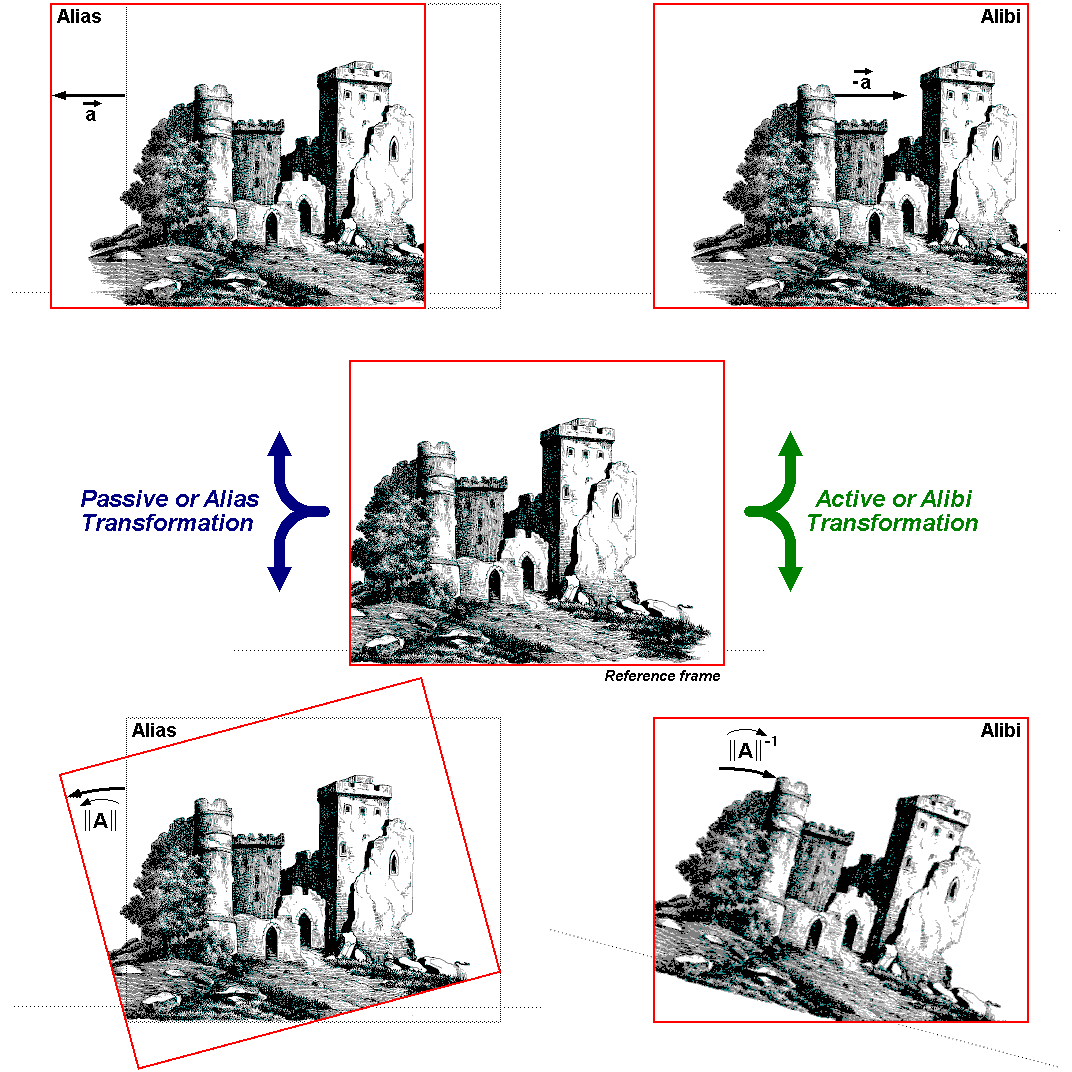
\includegraphics[width=3.5in]{../images/adjoint/alias_and_alibi.png}
\caption{A dual system and two pair of adjoint operators\cite{wiki:aatrans}}
\end{figure}

\begin{definition}
\label{d0}
A dual system $ \langle X, Y \rangle $ is a bilinear mapping $ \langle , \rangle : X \times Y \to F $ where $X$, $Y$ are two vector space and $ F $ is a field.
\end{definition}

\begin{definition}
\label{d1}
For two dual system $ \langle X_1, Y_1 \rangle $ and $ \langle X_2, Y_2 \rangle $ , each of the two operator $ A : X_1 \to X_2$ and $ B : Y_2 \to Y_1 $ is an adjoint of the other counterpart,
if and only if, the equation $$ \langle A \phi, \psi \rangle = \langle \phi, B \psi \rangle $$ holds for arbitrary $ \phi \in X_1 $ and $ \psi \in Y_2 $
\end{definition}

Geometrically, We can interpret $ X $ in $ \langle X, Y \rangle $ as bottom space, while $ Y $ is frame space, and the value of $ \langle x, y \rangle $ is a coordinate.
Under this interpretation, a pair of adjoint operators are just active and passive transformations (or alibi and alias transformations)\cite{wiki:aptrans}.

\subsection{The traditional way to introduce adjoint equation}

Adjoint equation is a tool when we seek an optimized solution bounded to an evolutionary process satisfying a differential equation, here the optimized solution can be a boundary value to apply control, or instead, an initial value to fit the observation aftermath, or possibly, better parameters to influence evolution. To handle all these different settings, we give a generalized formulation as below.

\section{Geometrical interpretation of adjoint equation}

\subsection{Additional and multiplicational point of view}

\subsection{Forward and backward propagation of a disturbance}

\subsection{The geometrical interpretation}


\section{Reformulate with dual number}


\section{Reformulate disturbance as a space}

the orbit of a disturbance is a point

\section{Applications}


\lipsum[8] \cite{Liberzon2012CalculusOV} and see \cite{hadash2018estimate}.

The documentation for \verb+natbib+ may be found at
\begin{center}
  \url{http://mirrors.ctan.org/macros/latex/contrib/natbib/natnotes.pdf}
\end{center}
Of note is the command \verb+\citet+, which produces citations
appropriate for use in inline text.  For example,
\begin{verbatim}
   \citet{hasselmo} investigated\dots
\end{verbatim}
produces
\begin{quote}
  Hasselmo, et al.\ (1995) investigated\dots
\end{quote}

\begin{center}
  \url{https://www.ctan.org/pkg/booktabs}
\end{center}


\subsection{Figures}
\lipsum[10] 
See Figure \ref{fig:fig1}. Here is how you add footnotes. \footnote{Sample of the first footnote.}
\lipsum[11] 

\begin{figure}
  \centering
  \fbox{\rule[-.5cm]{4cm}{4cm} \rule[-.5cm]{4cm}{0cm}}
  \caption{Sample figure caption.}
  \label{fig:fig1}
\end{figure}

\subsection{Tables}
\lipsum[12]
See awesome Table~\ref{tab:table}.

\begin{table}
 \caption{Sample table title}
  \centering
  \begin{tabular}{lll}
    \toprule
    \multicolumn{2}{c}{Part}                   \\
    \cmidrule(r){1-2}
    Name     & Description     & Size ($\mu$m) \\
    \midrule
    Dendrite & Input terminal  & $\sim$100     \\
    Axon     & Output terminal & $\sim$10      \\
    Soma     & Cell body       & up to $10^6$  \\
    \bottomrule
  \end{tabular}
  \label{tab:table}
\end{table}

\subsection{Lists}
\begin{itemize}
\item Lorem ipsum dolor sit amet
\item consectetur adipiscing elit. 
\item Aliquam dignissim blandit est, in dictum tortor gravida eget. In ac rutrum magna.
\end{itemize}


\bibliographystyle{unsrt}
\bibliography{references}

\end{document}
